\documentclass[11pt]{article}
\usepackage{graphicx,booktabs,geometry,hyperref}
\geometry{margin=22mm}
\title{Body-Fitted Finite-Volume External-Flow Verification}
\author{TensorFVM benchmark development}
\begin{document}\maketitle
\begin{abstract}
Actual steady laminar cylinder and NACA0012 calculations assess pressure, velocity and integrated traction on three polygon grids. Independent physical error gates are strictly below 3 percent. Numerical convergence, physical qualification and mesh convergence are reported separately; failures are retained.
\end{abstract}
\section{Physical problem and references}
The DFG 2D-1 cylinder has $Re=20$, diameter 0.1 m and channel size $2.2\times0.41$ m. Parabolic inlet mean velocity is 0.2 m/s. The FeatFlow references are $C_D=5.57953523384$, $C_L=0.010618948146$ and $\Delta p=0.11752016697$ Pa.
The NACA0012 has $Re=1000$, incidence 4 degrees, unit chord, and a $20\times16$ domain with leading edge at $(6,8)$.
Di Ilio et al. (2020), arXiv:2006.10487, figures 10 and 11 provide vector-digitized present-study markers $C_L=27.41/190.95\times1.4$ and $C_D=23.87/190.95$. Each carries a conservative graph-reading interval $\pm0.0001$, excluding author numerical uncertainty. Worst endpoint relative errors are used. The historical 0.205/0.120 reference and pass claim are withdrawn. No matching 4-degree tabulated $C_p$ reference is claimed.
\section{Numerical method and reproducibility}
Production collocated SIMPLE uses Rhie--Chow mass flux, first-order upwind momentum transport and nonorthogonal diffusion. CPU SuperLU solves identical sparse equations; CUDA optionally uses Torch Krylov. True linear residuals and final steady momentum, continuity and mass imbalance are checked. Circle and airfoil walls are polygon chords. The airfoil grid is periodic radial topology despite its c-grid API name. Owner pressure traction and a no-slip reconstructed molecular velocity gradient give body forces. Surface pressure is separately least-squares extrapolated for plots and cylinder pressure difference. No analytic solution initializes these external-flow fields.
Run the common module \texttt{tensorfvm.verification.external\_flow}; exact commands are in report.md. Raw NPZ fields, complete histories, metrics, per-solve residuals, source/artifact SHA256 and independent NumPy force audits are supplied. Five-step CPU/CUDA agreement is an auxiliary check only.
\section{Results}
\begin{tabular}{lrrrrl}\toprule Grid & Cells & Iterations & $C_D$ & $C_L$ & Qualified\\\midrule
64x24 & 1536 & 28 & 6.3247906 & 0.015101671 & False \\
128x48 & 6144 & 35 & 5.9720008 & 0.0097065854 & False \\
256x96 & 24576 & 33 & 5.8049572 & 0.0070831281 & False \\
\bottomrule\end{tabular}
\section{Fields, mesh and refinement}
\begin{figure}[p]\centering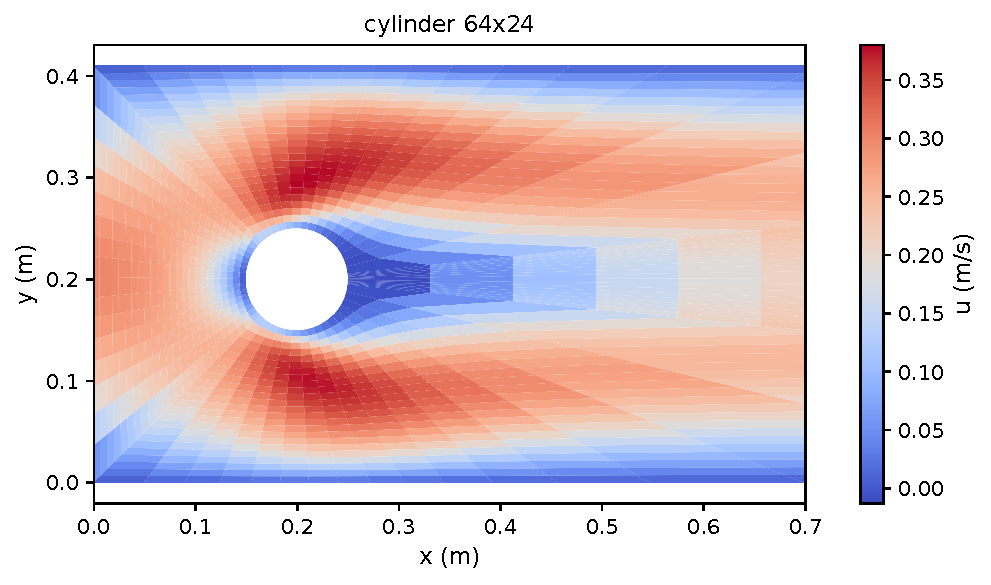
\includegraphics[width=.94\linewidth]{64x24/figures/u-component.pdf}\caption{64x24 figures u component}\end{figure}
\begin{figure}[p]\centering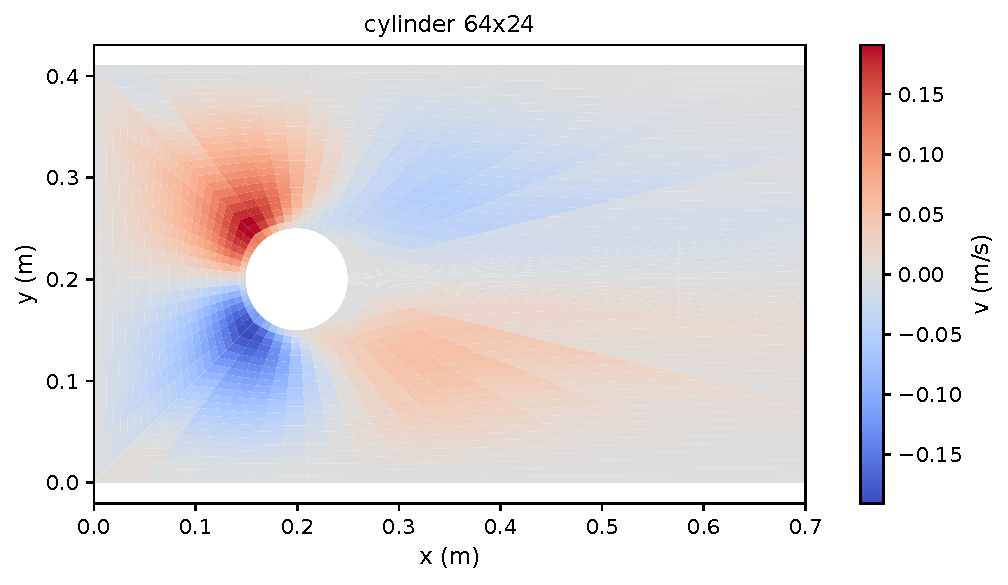
\includegraphics[width=.94\linewidth]{64x24/figures/v-component.pdf}\caption{64x24 figures v component}\end{figure}
\begin{figure}[p]\centering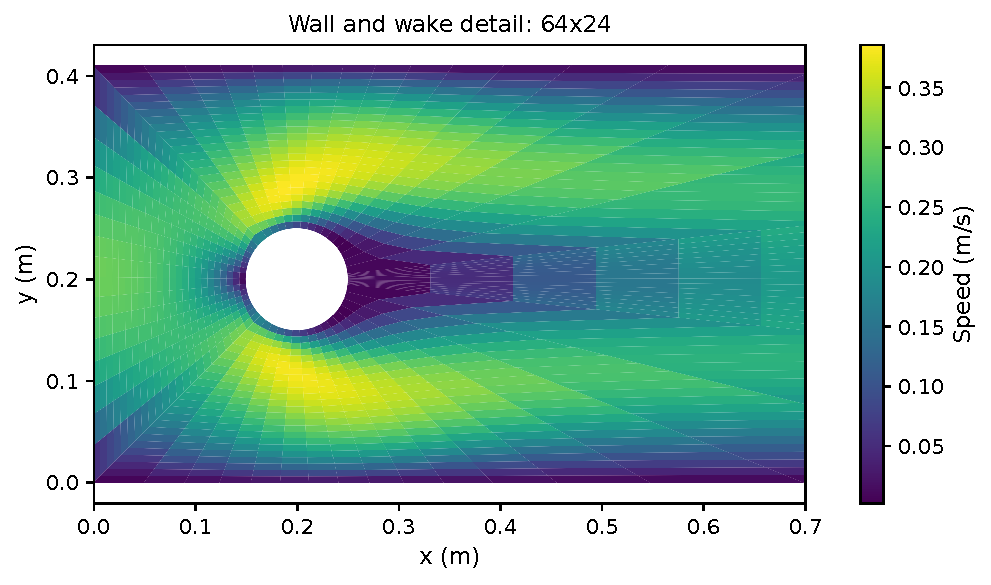
\includegraphics[width=.94\linewidth]{64x24/figures/wake-detail.pdf}\caption{64x24 figures wake detail}\end{figure}
\begin{figure}[p]\centering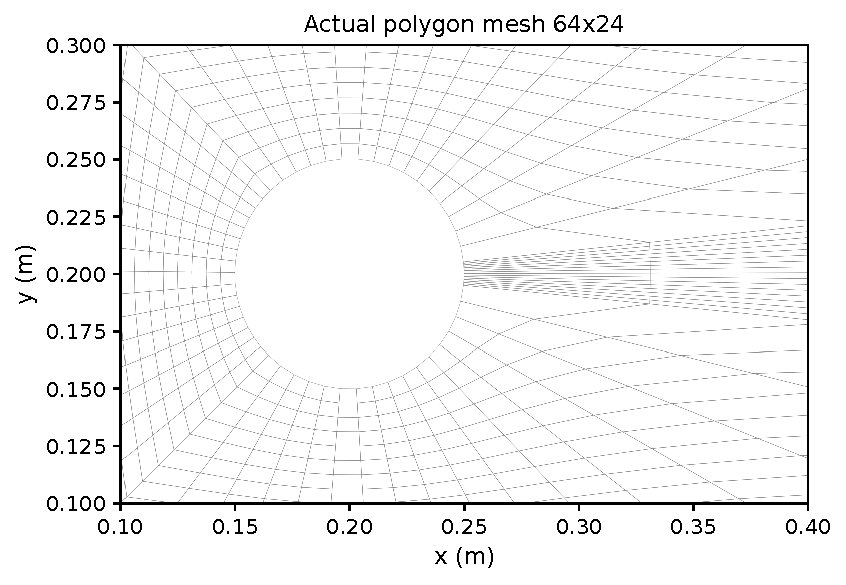
\includegraphics[width=.94\linewidth]{64x24/figures/mesh-detail.pdf}\caption{64x24 figures mesh detail}\end{figure}
\begin{figure}[p]\centering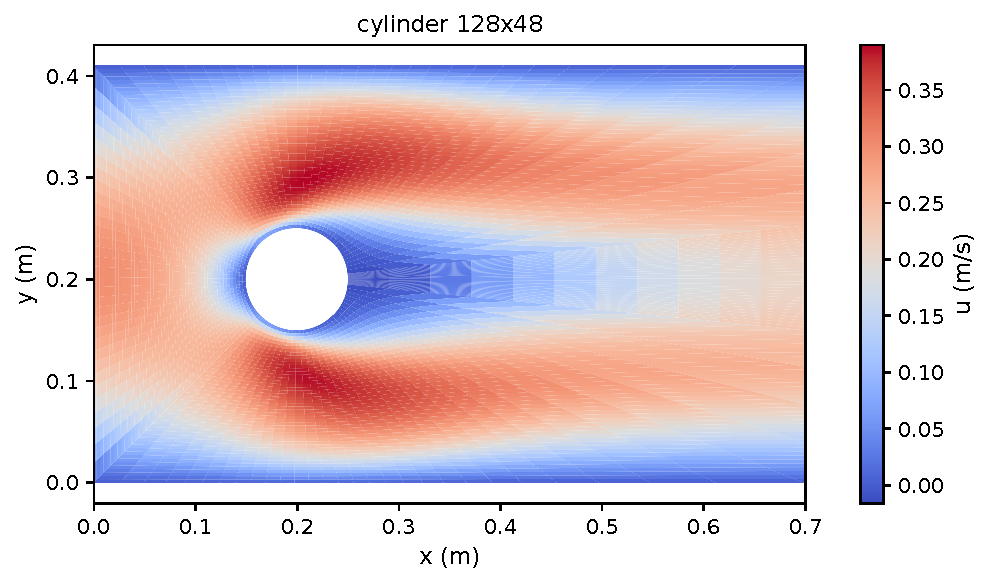
\includegraphics[width=.94\linewidth]{128x48/figures/u-component.pdf}\caption{128x48 figures u component}\end{figure}
\begin{figure}[p]\centering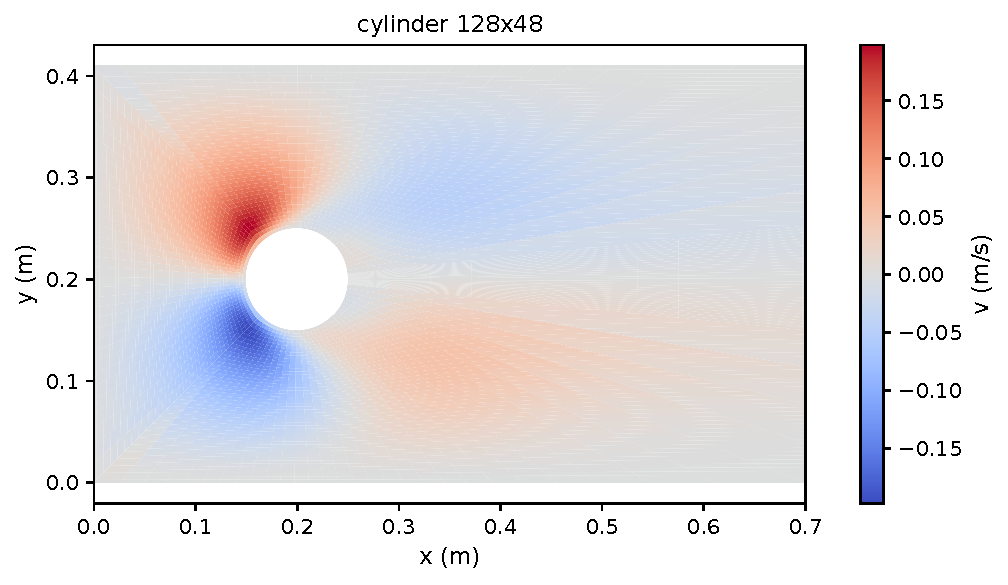
\includegraphics[width=.94\linewidth]{128x48/figures/v-component.pdf}\caption{128x48 figures v component}\end{figure}
\begin{figure}[p]\centering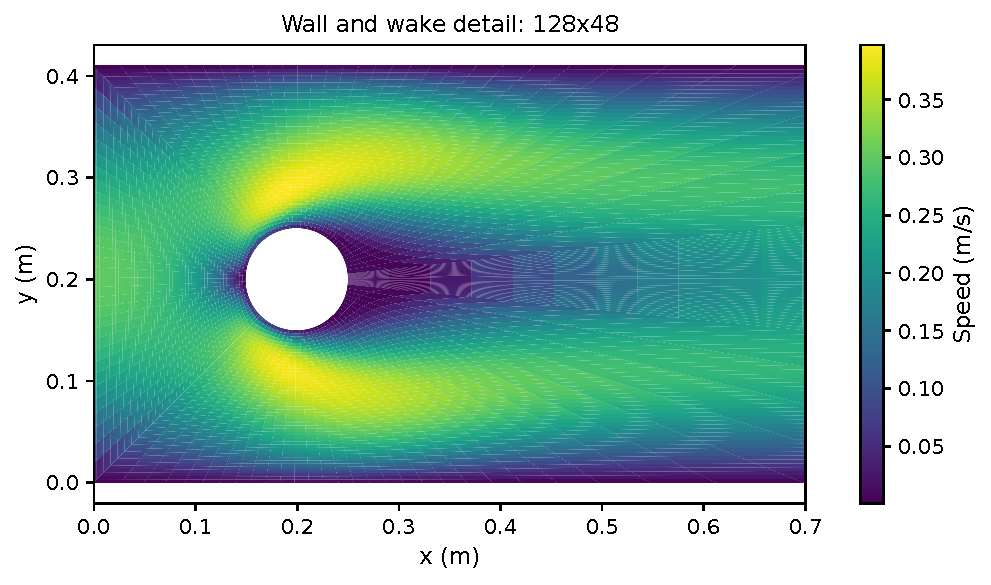
\includegraphics[width=.94\linewidth]{128x48/figures/wake-detail.pdf}\caption{128x48 figures wake detail}\end{figure}
\begin{figure}[p]\centering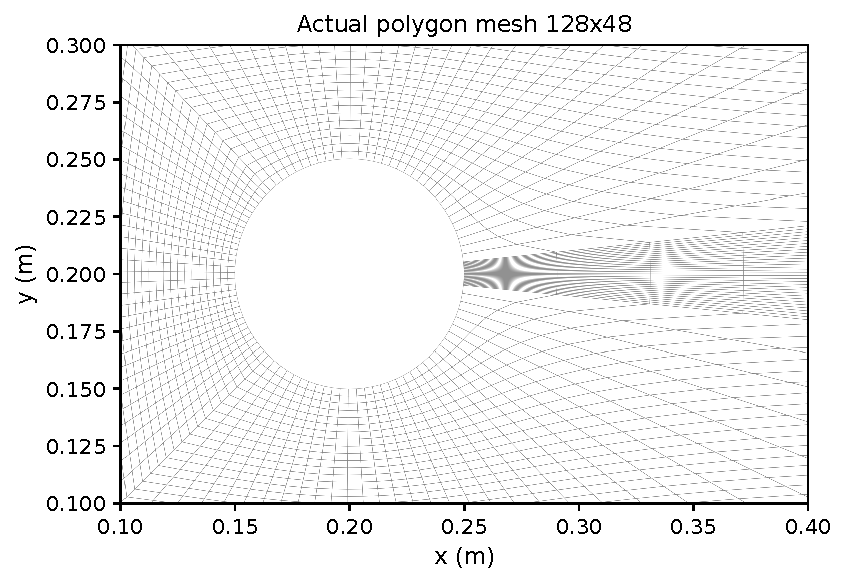
\includegraphics[width=.94\linewidth]{128x48/figures/mesh-detail.pdf}\caption{128x48 figures mesh detail}\end{figure}
\begin{figure}[p]\centering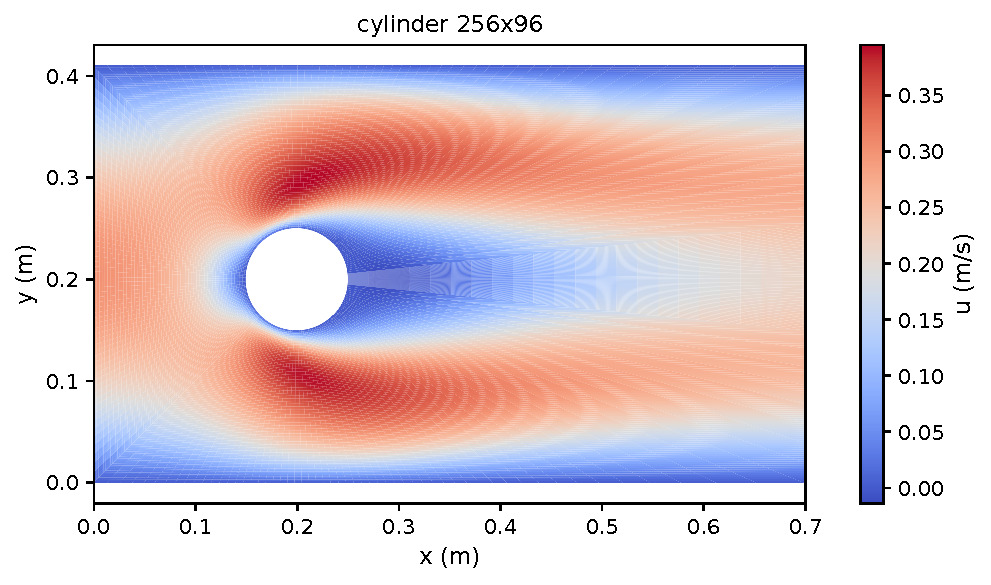
\includegraphics[width=.94\linewidth]{256x96/figures/u-component.pdf}\caption{256x96 figures u component}\end{figure}
\begin{figure}[p]\centering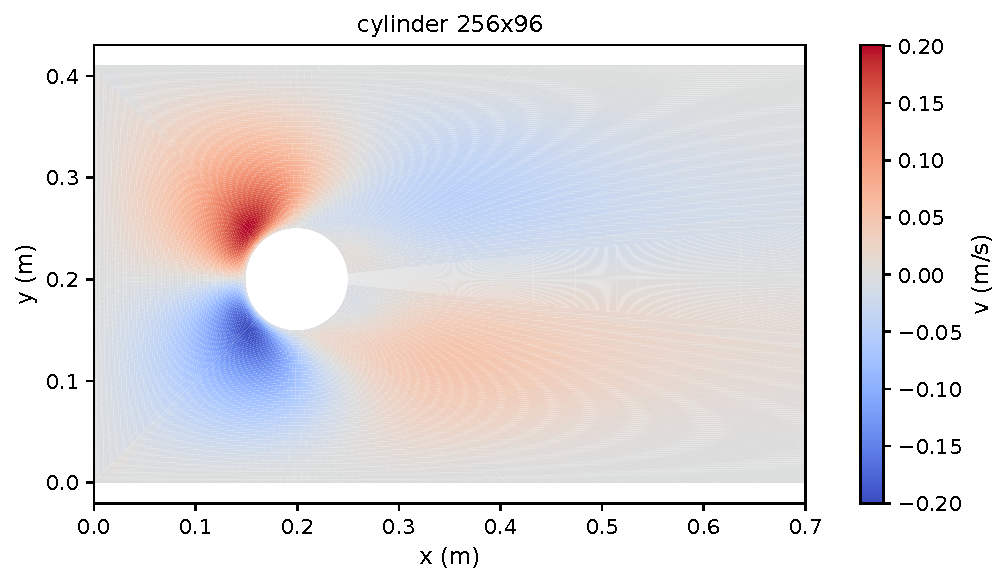
\includegraphics[width=.94\linewidth]{256x96/figures/v-component.pdf}\caption{256x96 figures v component}\end{figure}
\begin{figure}[p]\centering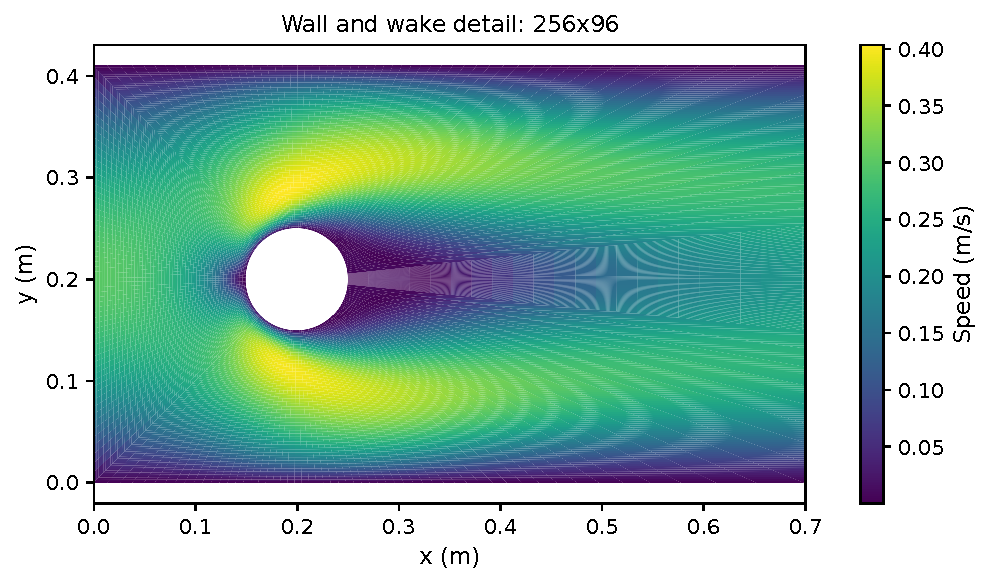
\includegraphics[width=.94\linewidth]{256x96/figures/wake-detail.pdf}\caption{256x96 figures wake detail}\end{figure}
\begin{figure}[p]\centering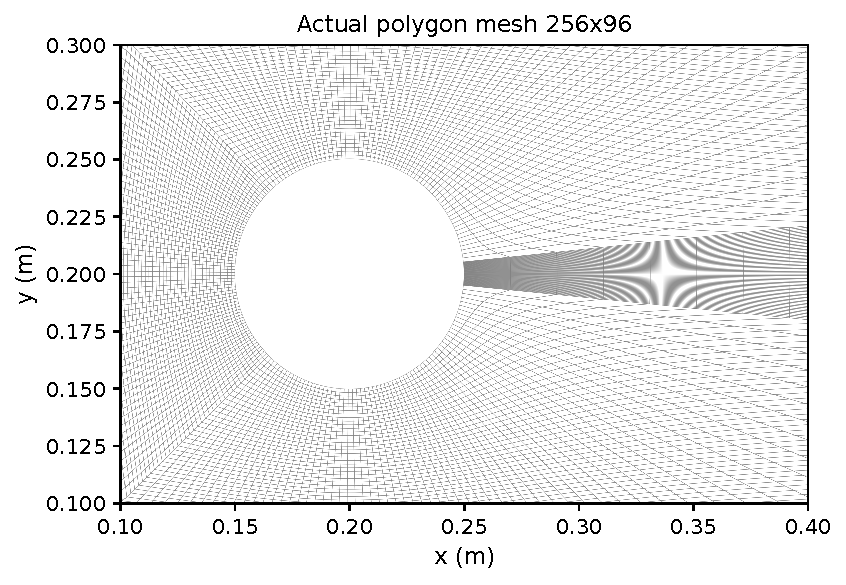
\includegraphics[width=.94\linewidth]{256x96/figures/mesh-detail.pdf}\caption{256x96 figures mesh detail}\end{figure}
\begin{figure}[p]\centering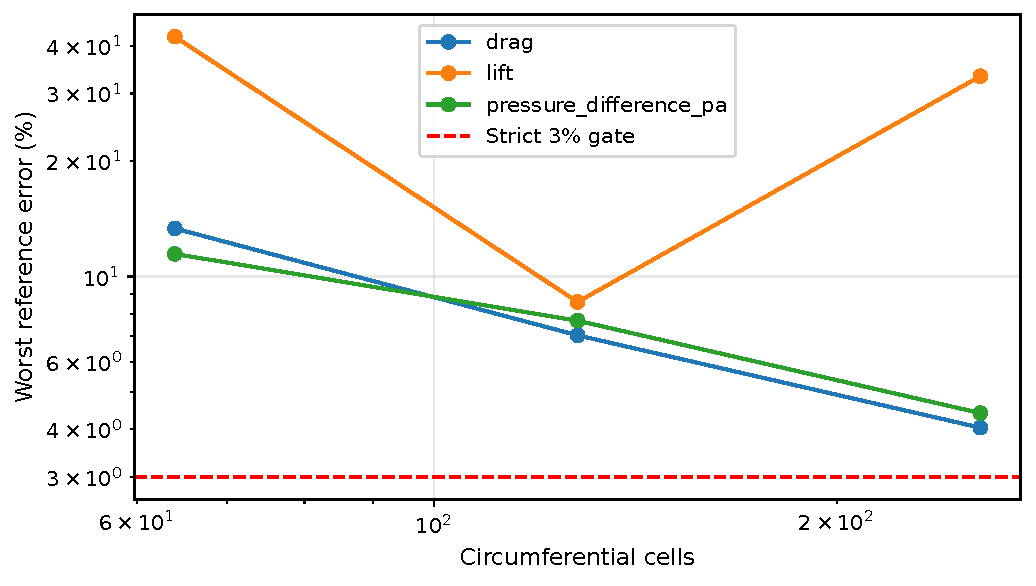
\includegraphics[width=.94\linewidth]{refinement.pdf}\caption{refinement}\end{figure}
\begin{figure}[p]\centering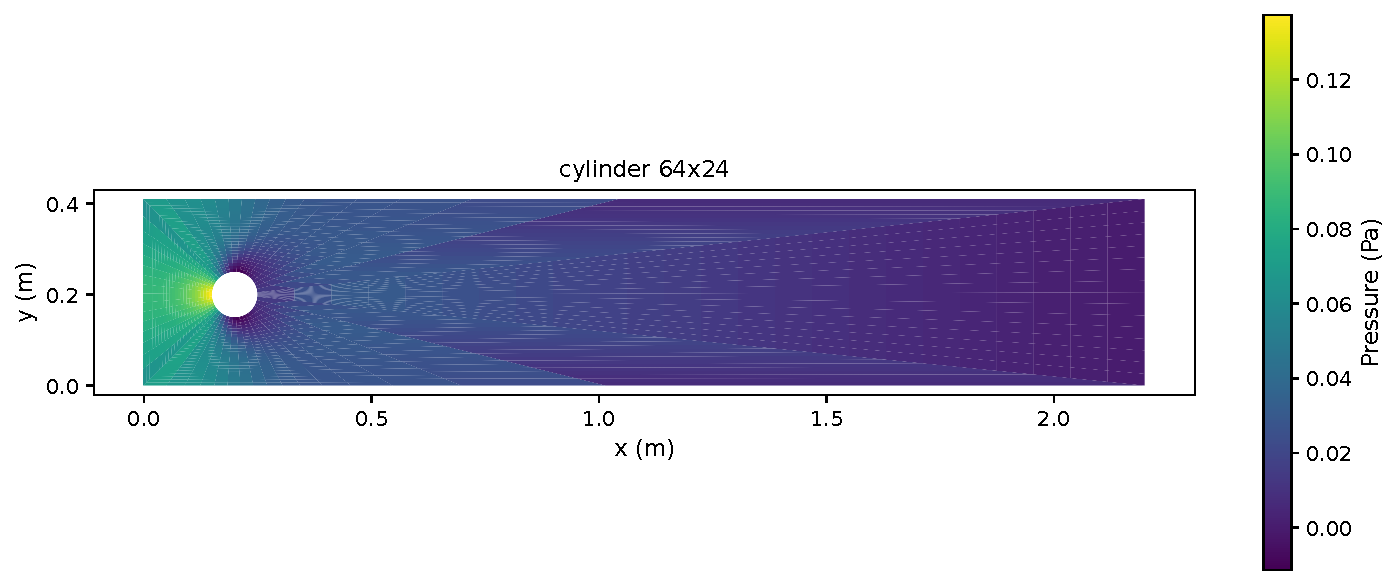
\includegraphics[width=.9\linewidth]{64x24/figures/pressure.pdf}\caption{64x24 pressure}\end{figure}
\begin{figure}[p]\centering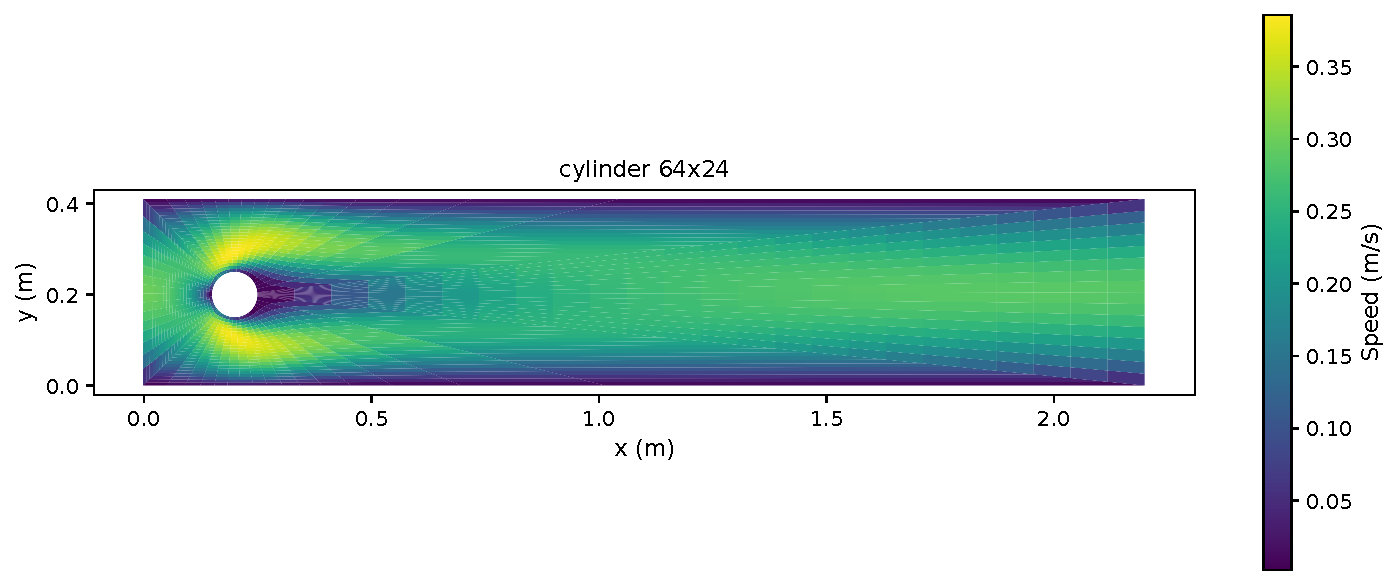
\includegraphics[width=.9\linewidth]{64x24/figures/velocity.pdf}\caption{64x24 velocity}\end{figure}
\begin{figure}[p]\centering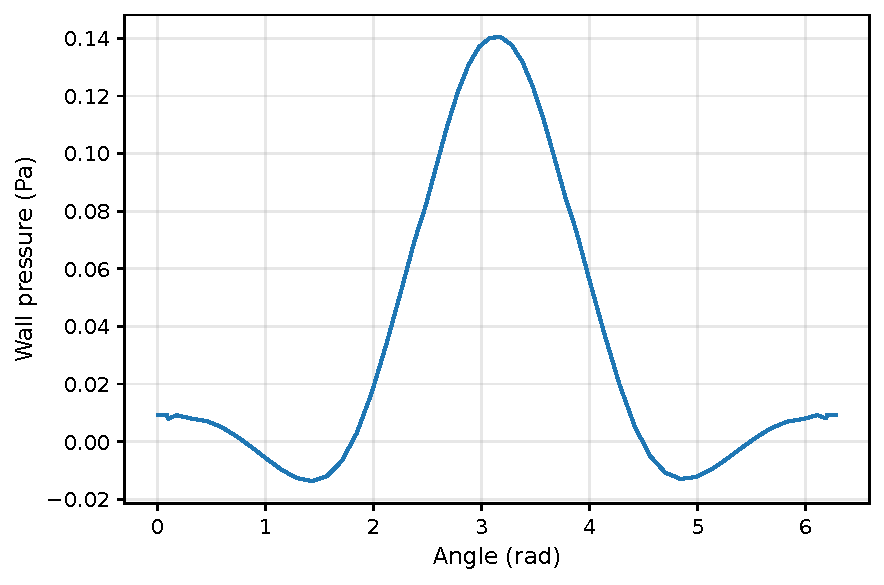
\includegraphics[width=.9\linewidth]{64x24/figures/surface-pressure.pdf}\caption{64x24 surface pressure}\end{figure}
\begin{figure}[p]\centering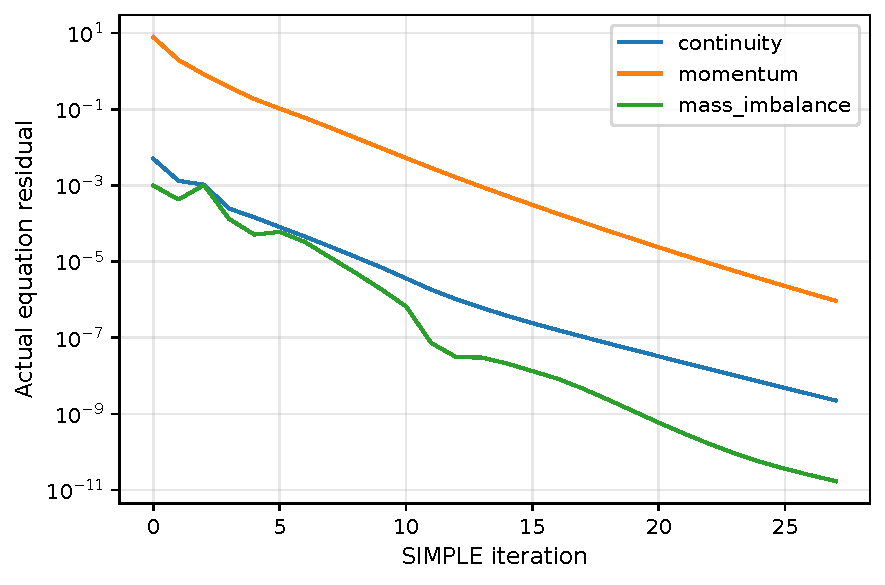
\includegraphics[width=.9\linewidth]{64x24/figures/residuals.pdf}\caption{64x24 residuals}\end{figure}
\begin{figure}[p]\centering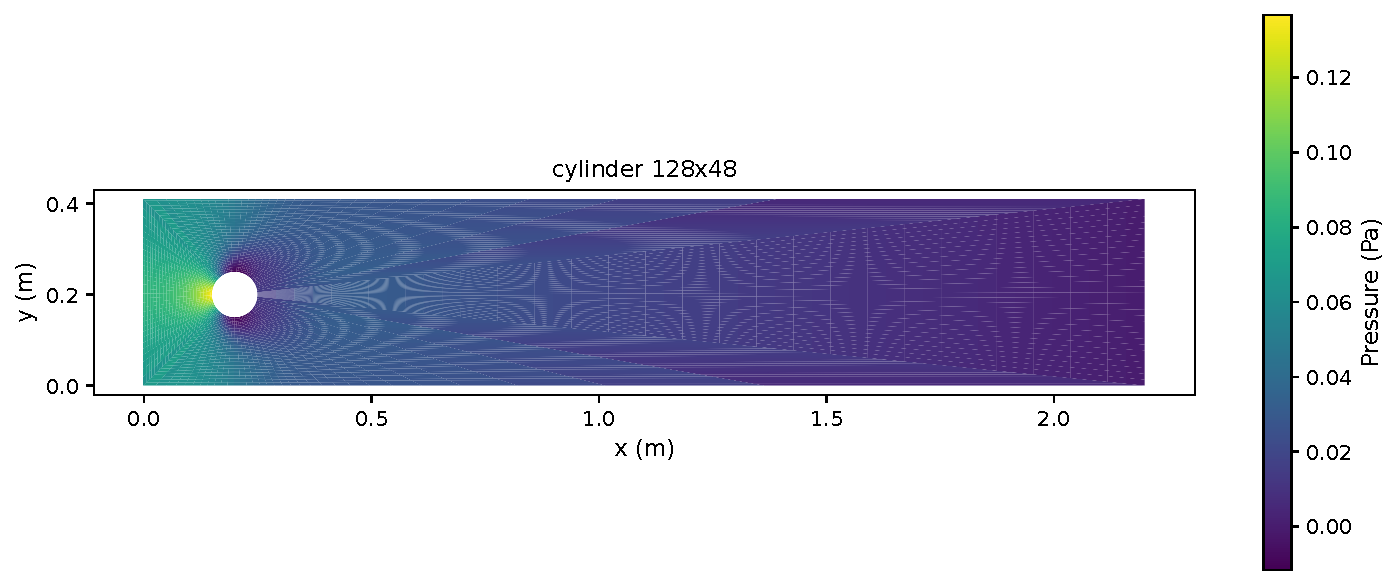
\includegraphics[width=.9\linewidth]{128x48/figures/pressure.pdf}\caption{128x48 pressure}\end{figure}
\begin{figure}[p]\centering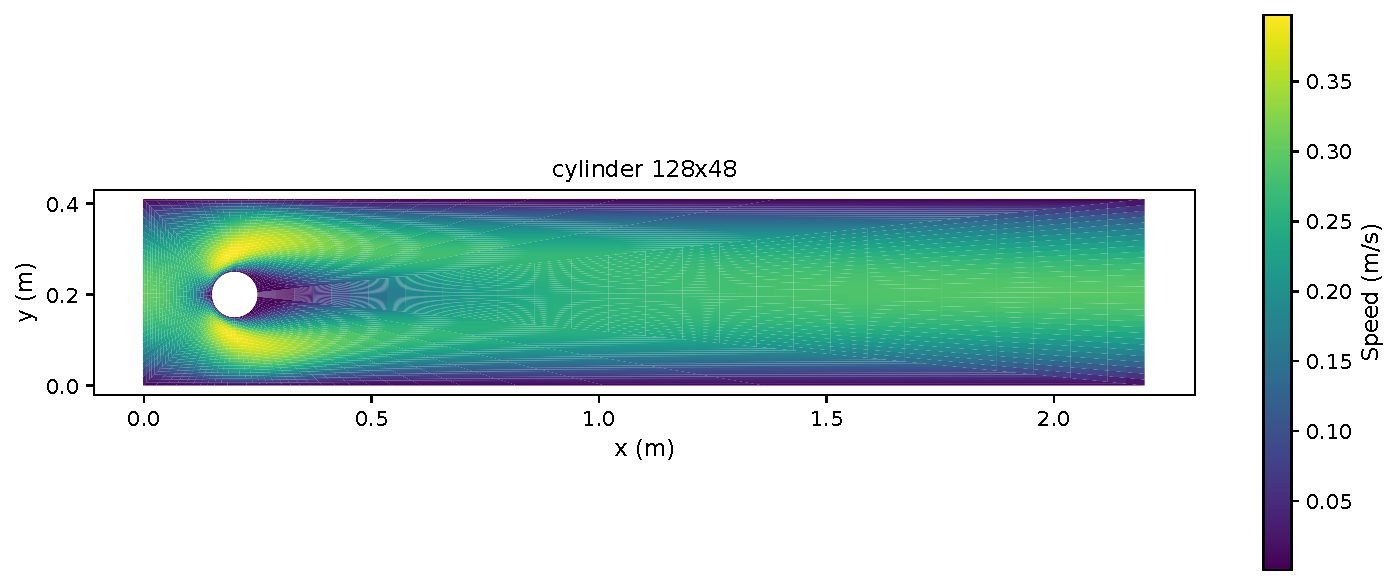
\includegraphics[width=.9\linewidth]{128x48/figures/velocity.pdf}\caption{128x48 velocity}\end{figure}
\begin{figure}[p]\centering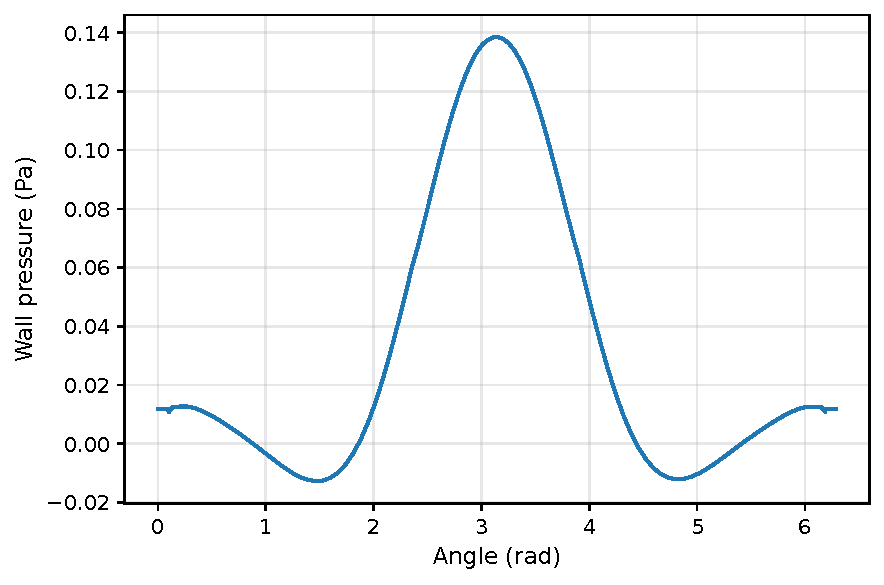
\includegraphics[width=.9\linewidth]{128x48/figures/surface-pressure.pdf}\caption{128x48 surface pressure}\end{figure}
\begin{figure}[p]\centering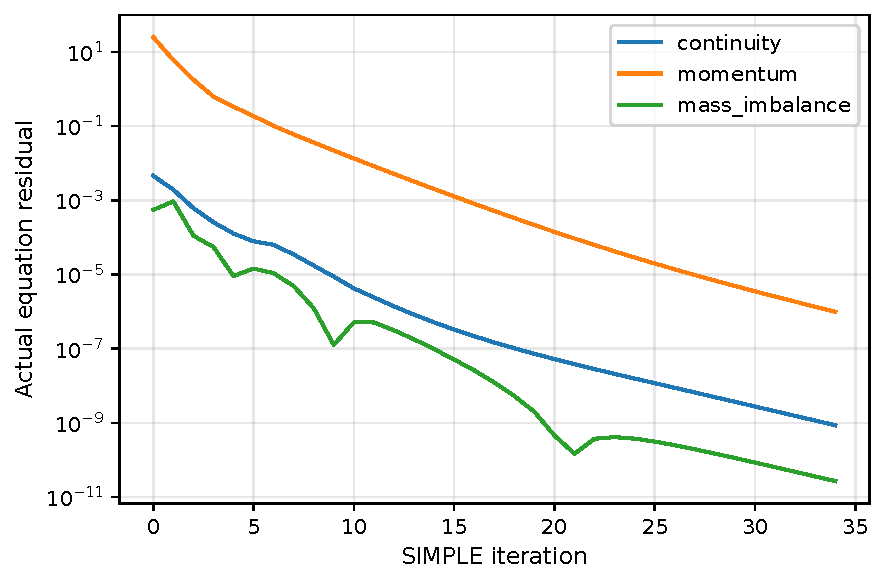
\includegraphics[width=.9\linewidth]{128x48/figures/residuals.pdf}\caption{128x48 residuals}\end{figure}
\begin{figure}[p]\centering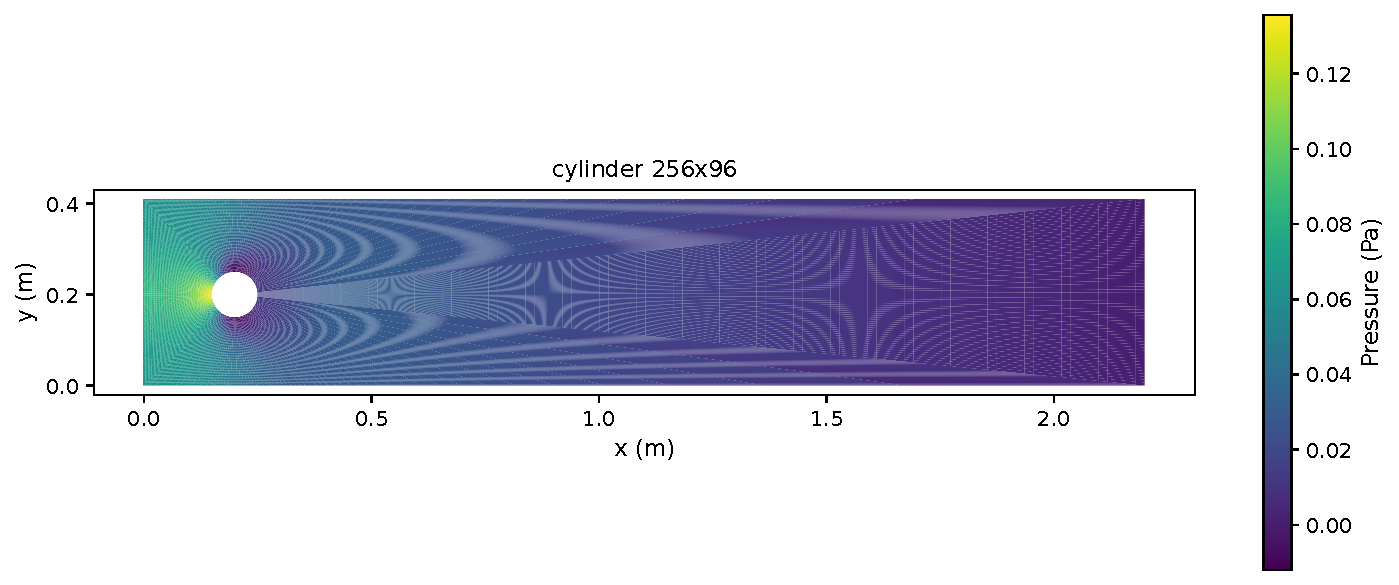
\includegraphics[width=.9\linewidth]{256x96/figures/pressure.pdf}\caption{256x96 pressure}\end{figure}
\begin{figure}[p]\centering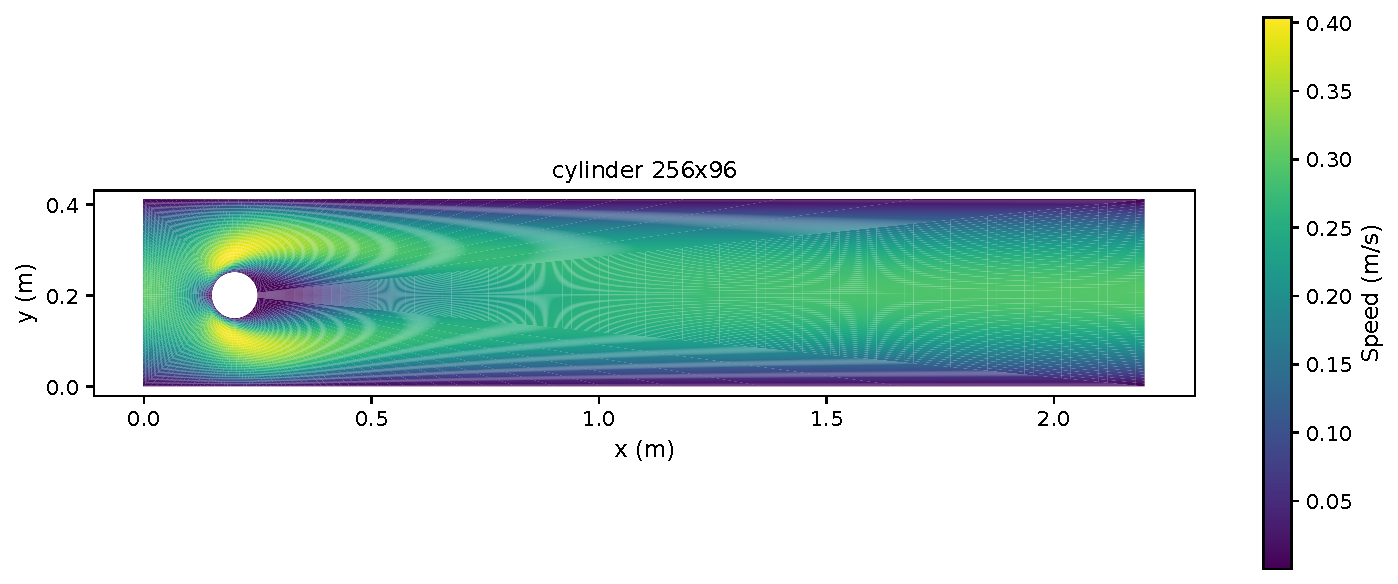
\includegraphics[width=.9\linewidth]{256x96/figures/velocity.pdf}\caption{256x96 velocity}\end{figure}
\begin{figure}[p]\centering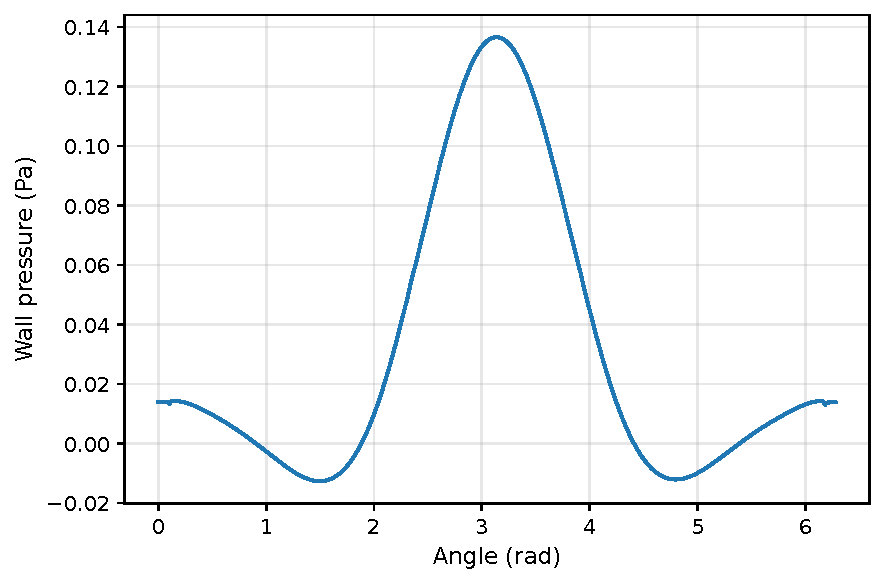
\includegraphics[width=.9\linewidth]{256x96/figures/surface-pressure.pdf}\caption{256x96 surface pressure}\end{figure}
\begin{figure}[p]\centering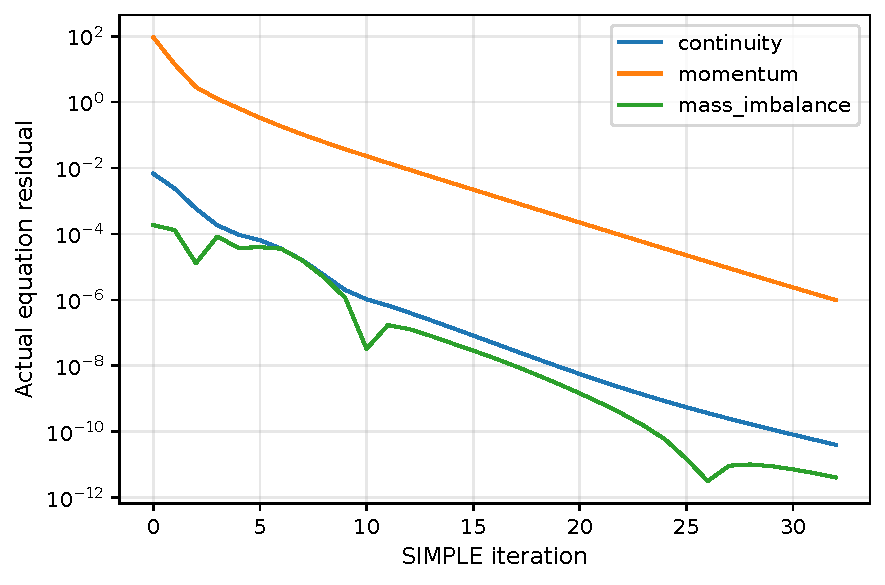
\includegraphics[width=.9\linewidth]{256x96/figures/residuals.pdf}\caption{256x96 residuals}\end{figure}
\section{Discussion and limits} Three resolutions do not automatically establish an asymptotic regime. First-order upwind, polygon geometry, wall traction and finite-domain effects remain candidates for error separation. No matched TensorLBM runs or performance ranking are claimed. This is steady two-dimensional laminar verification, not high-Reynolds-number shedding or industrial airfoil certification.\end{document}
